\subsection{HTB02 - Time}

    \subsubsection{Escaneo}
        \large{Como primera etapa de la Prueba de Penetración realizamos un escaneo de puertos abiertos en la máquina víctima con la herramienta "Nmap", donde se encuentran dos de ellos, el 22 con el servicio SSH y el 80 con un servidor web Apache.}
        \par
        \begin{figure}[H]
            \centering
            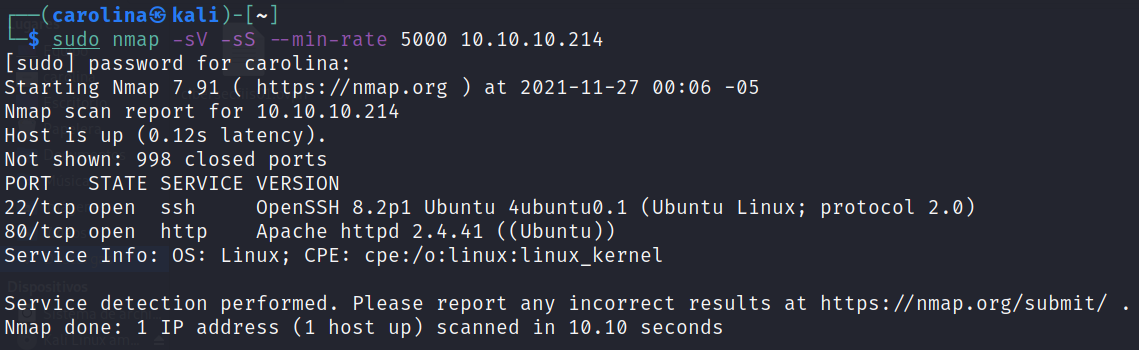
\includegraphics[width=0.99\textwidth]{imagenes/time/01_nmap_time.png} 
            \caption{Escaneo de puertos Time} 
        \end{figure}

    \subsubsection{Análisis de Vulnerabilidades}
    
        \large{Se procedió a revisar el sitio web, donde se encontró un combobox con las opciones de "butterfly" y "validate(beta)", junto con un recuadro de input, en el que si se escribía cualquier cosa en la cuando estaba en la opción "validate(beta)" mandaba un error de java, que al revisarlo completo se encuentra una exception y un "fasterxml.jackson".}
        \par
        \begin{figure}[H]
            \centering
            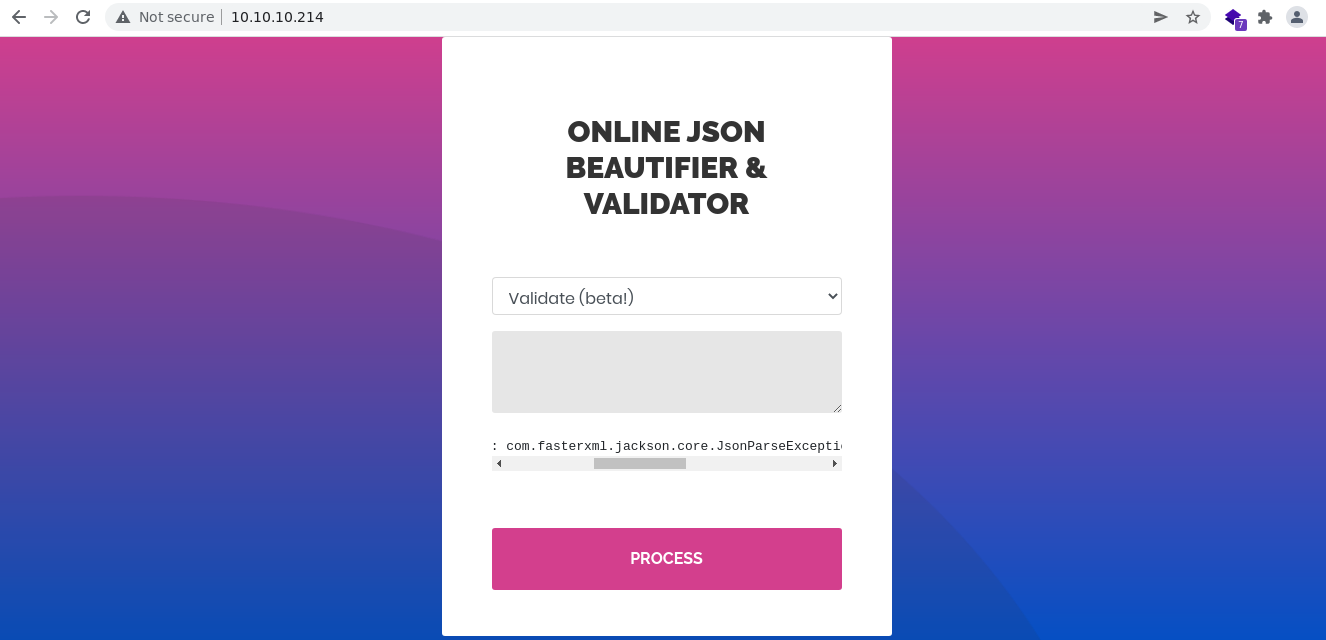
\includegraphics[width=0.99\textwidth]{imagenes/time/02_web_beta_time.png}
            \caption{Página Web Time}
        \end{figure}

        \large{Al investigar sobre "fasterxml.jackson", se relacionó con el CVE-2019-12384, vulnerabilidad que permite a los atacantes acceder a ejecutar la máquina víctima de forma remota y que tiene un exploit, el cual se visualiza en la imagen de abajo.}
        \par
        \begin{figure}[H]
            \centering
            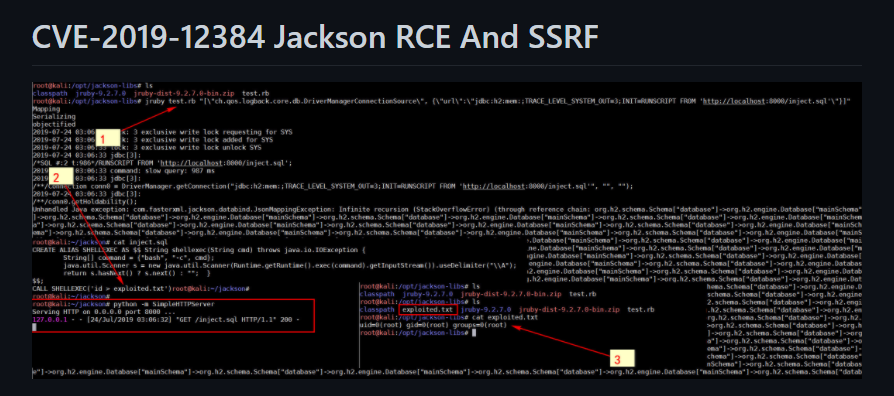
\includegraphics[width=0.99\textwidth]{imagenes/time/03_exploit_jackson.png}
            \caption{Exploit Jackson RCE y SSRF en Time}
        \end{figure}

    \subsubsection{Explotación}

        \large{Con el comando cat se revisó el inject.}
        \par
        \begin{figure}[H]
            \centering
            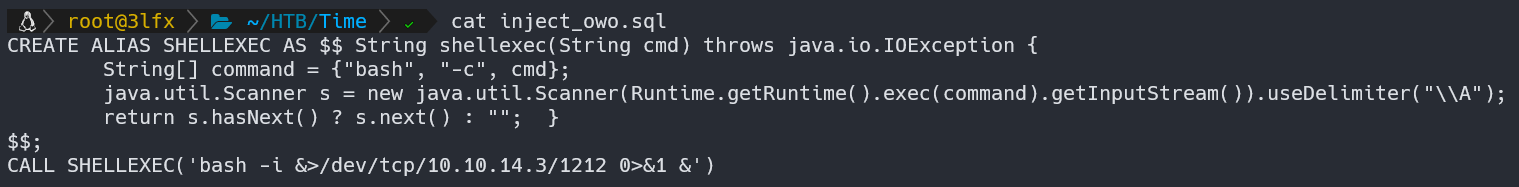
\includegraphics[width=0.99\textwidth]{imagenes/time/04_inject_time.png}
            \caption{Inject en Time}
        \end{figure}

        \large{Se copió y pegó en el input de la página web de Time, con la opción de "validate(beta)", la secuencia obtenida del inject.}
        \par
        \begin{figure}[H]
            \centering
            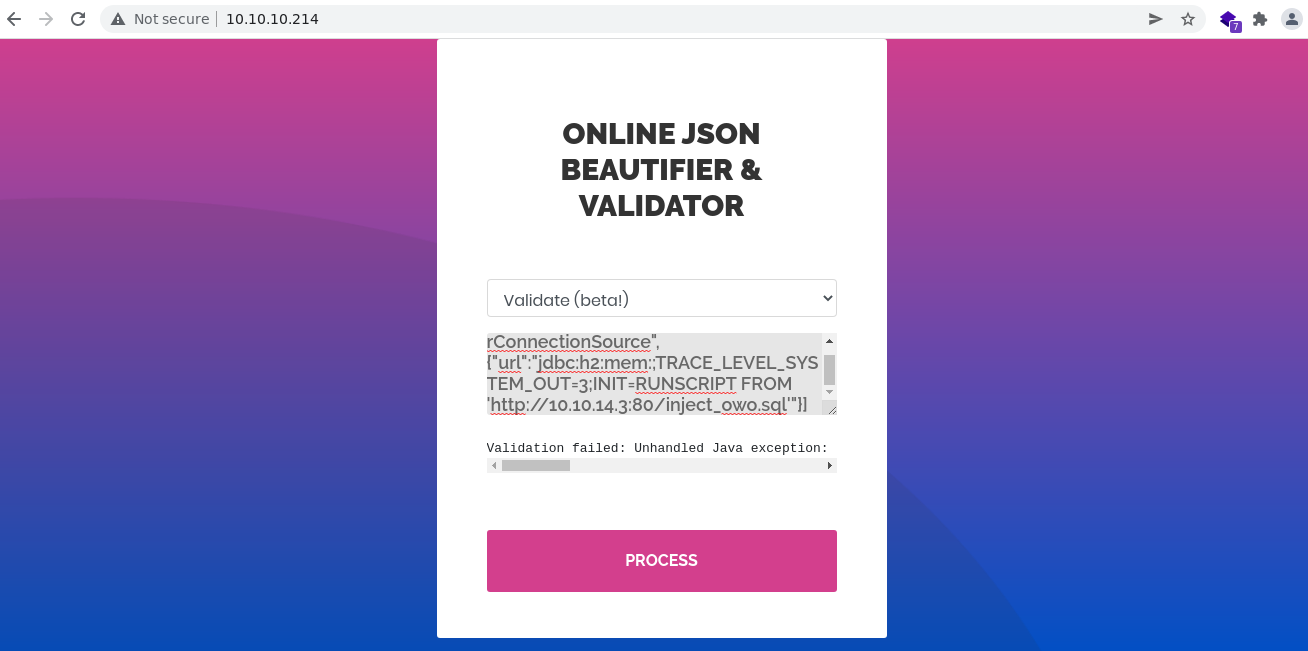
\includegraphics[width=0.99\textwidth]{imagenes/time/05_web_command_time.png}
            \caption{Comando inject en la web de Time}
        \end{figure}

        \large{Con python ejecutamos al http el inject, como s observa en la siguiente imagen.}
        \par
        \begin{figure}[H]
            \centering
            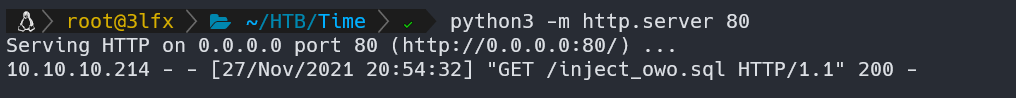
\includegraphics[width=0.99\textwidth]{imagenes/time/06_http_inject_time.png}
            \caption{Http Inject en Time}
        \end{figure}

        \large{Establecemos el puerto de escucha y en la imagen de abajo se puede apreciar que se estableció la conección con el usuario "pericles".}
        \par
        \begin{figure}[H]
            \centering
            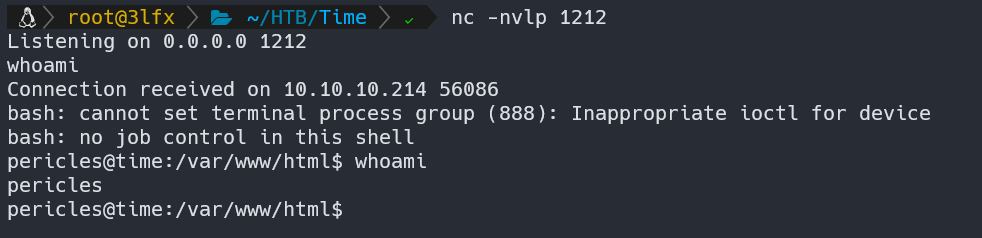
\includegraphics[width=0.99\textwidth]{imagenes/time/07_conect_pericles_time.png}
            \caption{Http Inject en Time}
        \end{figure}

    \subsubsection{Escalamiento de Privilegios}

        \large{Revisando los archivos a los que el usuario "pericles" tiene acceso, encontramos el archivo "user.txt", el cual cuenta con la flag.}
        \par
        \begin{figure}[H]
            \centering
            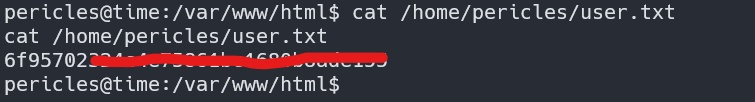
\includegraphics[width=0.99\textwidth]{imagenes/time/08_user_flag_time.jpg}
            \caption{User flag en Time}
        \end{figure}

        \large{Ahora tratamos de escalar privilegios en la máquina, para ello listamos los archivos binarios con permiso SUID, como se aprecia en la siguiente imagen.}
        \par
        \begin{figure}[H]
            \centering
            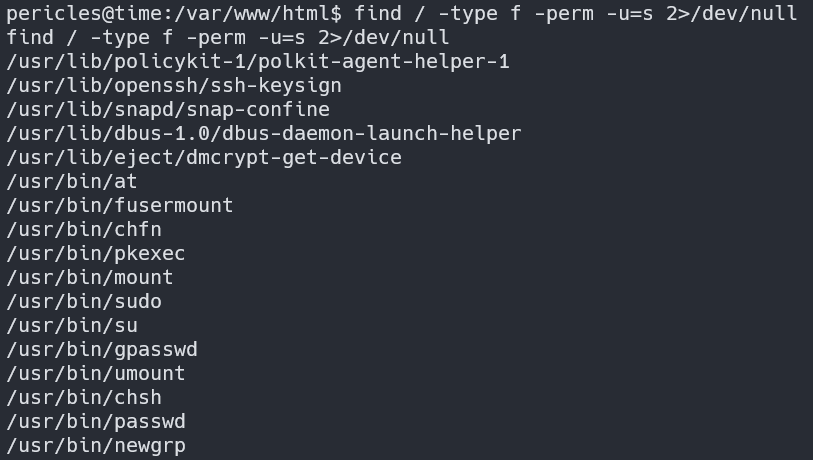
\includegraphics[width=0.99\textwidth]{imagenes/time/09_bin_suid_time.png}
            \caption{Archivos binarios en Time}
        \end{figure}

        \large{Al no encontrar niguno que conicida con la documentación base que se utilizó en la máquina anterior, se decidió revisar los grupos de archivos, los cuales se listan en la siguiente imagen.}
        \par
        \begin{figure}[H]
            \centering
            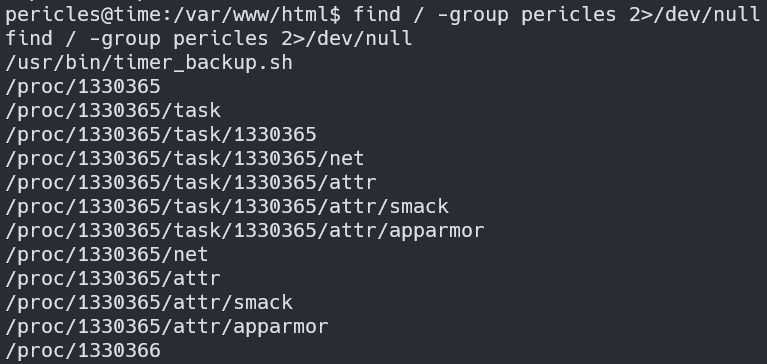
\includegraphics[width=0.99\textwidth]{imagenes/time/10_files_group_time.png}
            \caption{Grupos de archivos en Time}
        \end{figure}

        \large{Revisando el archivo timer-backup encontramos un archivo .zip con el nombre root/backup.}
        \par
        \begin{figure}[H]
            \centering
            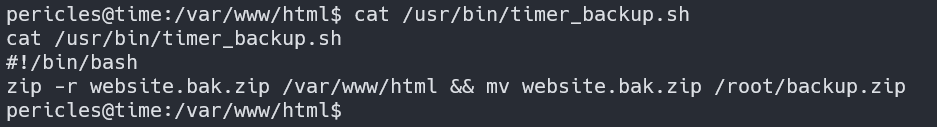
\includegraphics[width=0.99\textwidth]{imagenes/time/11_timer_backup_code.png}
            \caption{Timer backup code en Time}
        \end{figure}

        \large{Con el comando grep buscamos dentro del archivo la información que necesitamos como se aprecia en la imagen.}
        \par
        \begin{figure}[H]
            \centering
            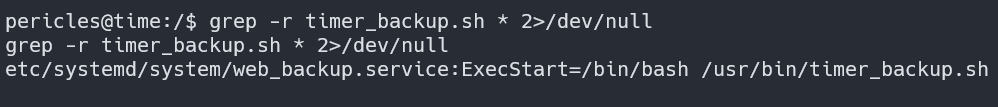
\includegraphics[width=0.99\textwidth]{imagenes/time/12_grep_timer_sh.png}
            \caption{Grep em timer-backup en Time}
        \end{figure}

        \large{Listamos el service web-backup.}
        \par
        \begin{figure}[H]
            \centering
            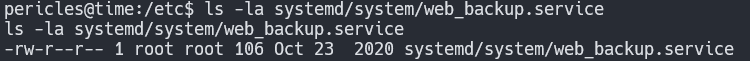
\includegraphics[width=0.99\textwidth]{imagenes/time/13_perm_service_backup.png}
            \caption{Service backup en Time}
        \end{figure}

        \large{Se otorgan permisos ssh a la máquina atacante, de la siguiente manera.}
        \par
        \begin{figure}[H]
            \centering
            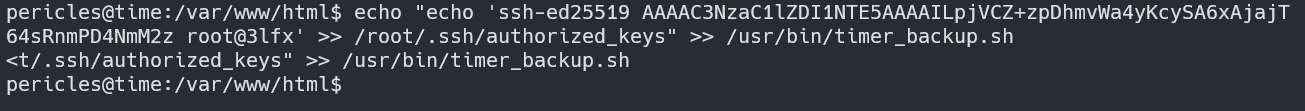
\includegraphics[width=0.99\textwidth]{imagenes/time/14_ssh_authorized_time.png}
            \caption{Autorización ssh en Time}
        \end{figure}

        \large{Especificamos las cles de ssh y logramos el acceso con usuario root, como se evidencia en la imagen de abajo.}
        \par
        \begin{figure}[H]
            \centering
            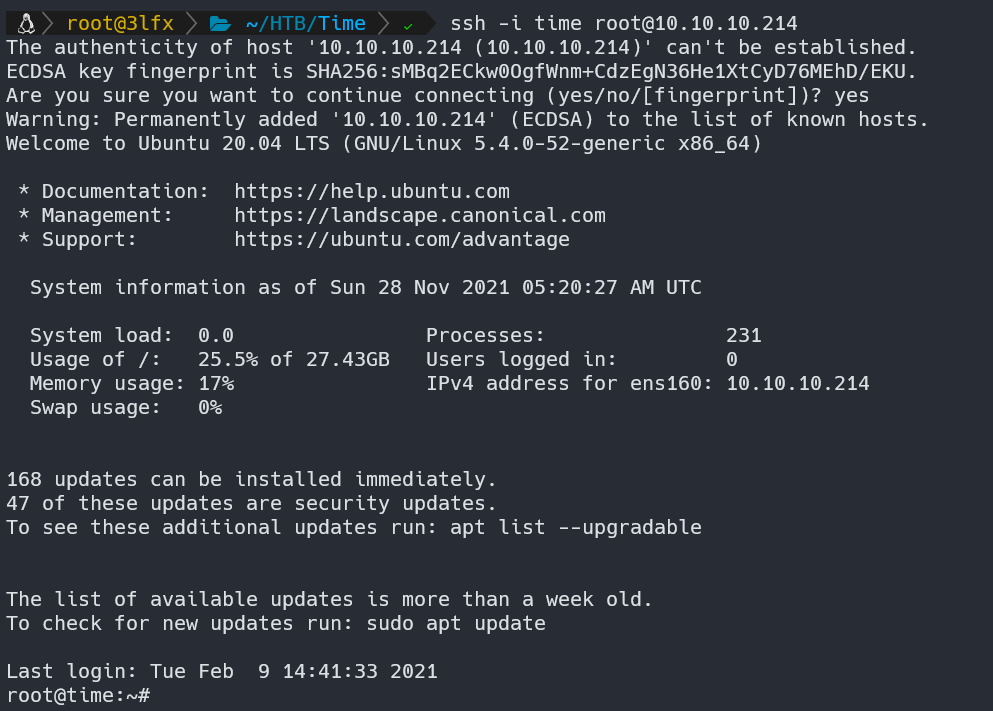
\includegraphics[width=0.99\textwidth]{imagenes/time/15_conect_root_time.png}
            \caption{conexion root en Time}
        \end{figure}

        \large{Revisando los archivos a los que se tiene ahora acceso, encontramos el archivo "root.txt", donde se ubica la flag.}
        \par
        \begin{figure}[H]
            \centering
            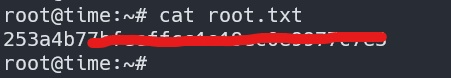
\includegraphics[width=0.99\textwidth]{imagenes/time/16_root_flag_time.jpg}
            \caption{Root flag en Time}
        \end{figure}

    \subsubsection{Post-Explotación}

        \large{Para la post-explotación se procede a extraer los hashes pertenecientes a los usuarios del sistema.}
        \par
        \begin{figure}[H]
            \centering
            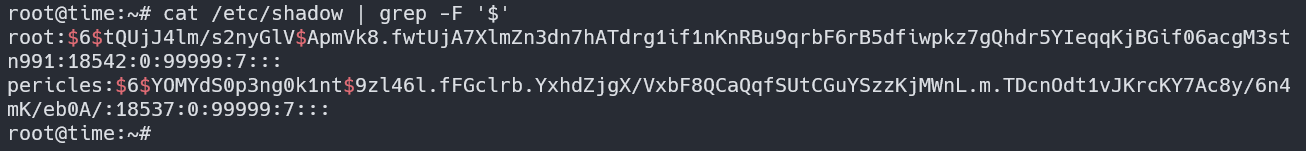
\includegraphics[width=0.99\textwidth]{imagenes/time/17_hashes_time.png}
            \caption{Hashes de Time}
        \end{figure}

    \subsubsection{Recomendaciones de Mitigación}

    \large{Para mitigar los ataques a la vulnerabilidad hallada en FasterXML jackson-databind se recomienda:}
    \begin{itemize}
        \item Actualizar a la versión 2.9.9.1 o a la más reciente de jackson-databind
        \item Desactivar el 'enableDefaultTyping' para una solución temporal
    \end{itemize}
